\documentclass[a4paper,11pt]{article}

\usepackage[utf8]{inputenc} % allow utf-8 input
\usepackage{hyperref}       % hyperlinks
\usepackage{url}            % simple URL typesetting
\usepackage{booktabs}       % professional-quality tables
\usepackage{amsfonts}       % blackboard math symbols
\usepackage{nicefrac}       % compact symbols for 1/2, etc.
\usepackage{microtype}      % microtypography
\usepackage{graphicx}       % include graphics
\usepackage{subcaption}     % subfigures
\usepackage{float}          % placement of floats
\usepackage{fancyhdr}       % head notes and foot notes
\usepackage{bbm}            % Nice symbols
\usepackage{mathtools}      % Math tools like operators
\graphicspath{ {images/} }



\newcommand{\RR}{\mathbbm{R}} % Nice R sign
\DeclarePairedDelimiter\abs{\lvert}{\rvert} % abs
\DeclarePairedDelimiter\norm{\lVert}{\rVert} % norm

\title{P3 - Dictionary learning, application to denoising and inpainting}


\author{
  Louis Martin\\
  \href{mailto:louis.martin@student.ecp.fr}{\tt louis.martin@student.ecp.fr}
}

\pagestyle{fancy}
\fancyhf{}
\lhead{Louis MARTIN}
\rhead{Sparsity and Compressed Sensing: Project}

\rfoot{Page \thepage}

\begin{document}

\maketitle

\begin{abstract}
%% Abstract (½ page):
%% What problem(s) is studied ?
This paper will focus on how to efficiently learn a dictionary in order to obtain a sparse representation of a signal (e.g. image or audio).
%% Why is it relevant ?
Deriving a sparse representation of a signal can be very efficient in solving multiple signal processing problems.
It has been successfully used in compression, inpainting, denoising, inverse problems and more.
One way to obtain a sparse coding is by using dictionaries.
A dictionary acts as a basis on which the data can be accurately represented using a small number of coefficients.
This basis can be either predefined or learned, both approaches have shown great results.
We will here focus how to efficiently learn an appropriate dictionary given the data we want to encode.
Finding a good dictionary is important because it will define the representational power of the sparse coding,
i.e. how well the sparse coded signal will represent the original signal.
The learning process is therefore a key step for sparse representation.
% TODO:
%% What solution(s) is proposed ?
%% Which contributions (theory, numerics, etc) ?

\end{abstract}

\section{Introduction}
%% Introduction (~3 pages) :
%% Presentation of the problem(s).
Sparse coding is able to solve multiple signal processing tasks such as compression, inpainting, denoising, texture synthesis and so on.
% Why do we want sparsity, i.e. a small number of non-zero coefficients ?
% 1) Compression
We want sparsity, i.e. a small number of non-zero coefficients for compression for obvious reasons of storage space.
% 2) Theorem in the first lecture -> good compression coefficients => good denoising
Good compression coefficients is also often implies good denoising properties.
Indeed noise is often small local high frequency information that pruned by the sparse coding.
% 3) Natural images tend to have a small number of non-zero coefficients.
% Complex images like random images (or lot of noise) or trees will have a higher number of coefficient.
Natural image also tend to have a small number of non-zero coefficient whereas complex images like
random images of images with trees will have a higher number of coefficients.
% Sparsity is the a good indicator of natural images
Sparsity is therefore a good indicator of natural images
%% Previous works (at least a few citations). If relevant, include things that you have seen during the MVA course (or possibly other courses).
The choice of the space in which the sparse representation lives is thus important.
The problem is often reduced to finding a good basis for this space.
It can be either be predefined or learned.

One can use a predefined basis which will be the same for all tasks and datasets such as the Fourier basis or the wavelet basis \cite{mallat1999}.
The fact that these basis do not depend on the data makes it hard to design but also powerful.
The good sparse representation of natural images in the wavelet space led to the success of the JPEG2000 algorithm for image compression \cite{marcellin00}.

Another approach is to learn the basis, i.e. to learn a dictionary which gives good results in several tasks. Indeed having a specific dictionary that can be adapted to certain type of images or to one image in particular can be very powerful.
The sparse representation can be sparser and at the same time representing the data better.
The term basis to denote an over complete dictionary is abusive. The atoms composing the dictionary are not linearly independent.
Instead of being harmful, designing overcomplete dicionaries gives more flexibility to the sparse representation and leads to easier problems.
% TODO:
%% Contributions. Why is the studied method different/better/worse/etc. than existing previous works.

\section{Problem statement}
\subsection{Notations}
Given a signal of size $m$, $y \in \RR^m$, a dictionary is a collection of $k$ prototype signal atoms represented in a matrix $D \in \RR^{m \times k}$
We want to find $x \in \RR^k$, the sparse representation of $y$ in the dictionary $D$.
We want an exact representation $D x = y$ or more frequently an approximate representation $y \approx D x$.
A sparse vector is a vector with a "small" number of non-zero coefficient.
The sparsity measure is the $l_0$ pseudo-norm denoted $\norm{.}_0$.
The sparsity constraint is hence $\norm{x}_0<N$ with $N \in \mathbbm{N}$.

The problem we want to solve is therefore
\begin{equation*}
\min\limits_{D \in \RR^{m \times k}, x \in \RR^k} \norm{y - Dx}_2  \text{ subject to } \norm{x}_0<N
\end{equation*}
Finding the best sparse representation of a signal is a NP-Hard problem, that is why we will approximate the signal.
The sparsity measure is the $l_0$ norm



\subsection{Finding the sparse representation}
MP OMP FOCUSS \cite{gorodnitsky97} PGD
Wikipedia -> A popular extension of Matching Pursuit (MP) is its orthogonal version: Orthogonal Matching Pursuit[11][12] (OMP). The main difference from MP is that after every step, all the coefficients extracted so far are updated, by computing the orthogonal projection of the signal onto the set of atoms selected so far. This can lead to better results than standard MP, but requires more computation.
\subsection{Finding the dictionary}
PGD MOD

% TODO: citation with author and date
% TODO: talking of 'basis' is abusive because it is often overcomplete
%%%%%%%%%% Taken from \cite{matrixfactorization}
%recently led to state-of-the-art
%results in numerous low-level signal processing tasks such as image denoising (Elad and Aharon,
%2006; Mairal et al., 2008b), texture synthesis (Peyre, 2009) and audio processing (Grosse et al.,
%2007; Fevotte et al., 2009; Zibulevsky and Pearlmutter, 2001), as well as higher- level tasks such as
%image classification (Raina et al., 2007; Mairal et al., 2008a, 2009b; Bradley and Bagnell, 2009;
%Yang et al., 2009),
%%%%%%%%%%
%The learnt basis look like wavelets / Gabor filters but are tuned to the data -> better accuracy
Not penilizing the dictionary -> dictionary values will increase for the sparse coef to tend to 0
\cite{olshausen97} (k-SVD p-4313 [24]).
\section{Dictionary learning methods}
%% Main body (~10 pages) :
%% Presentation of the method(s).
%% Theoretical guarantees.
%% Numerics.
Most of the iterative methods are composed of the two steps defined above.
Sparse coding the vector and updating the dictionary given this sparse representation.
\subsection{Block coordinare projected gradient descent}
\cite{olshausen97} (k-SVD p-4313 [24])
$$D^{(n+1)} = D^{(n)} - \tau (D^{(n)}X - Y) X^T$$
\begin{figure}[!htbp]
\centering
  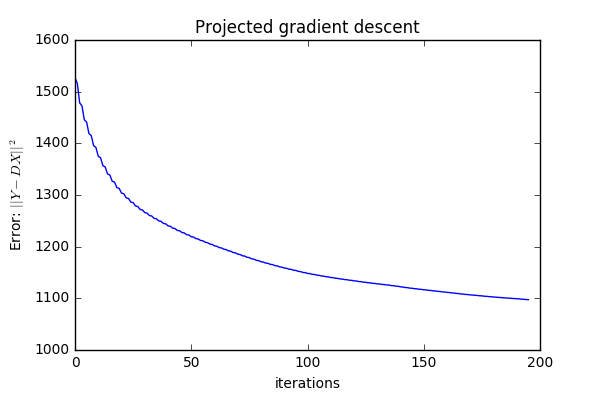
\includegraphics[width=\linewidth]{projected_gradient_descent.png}
\end{figure}
\subsection{Online learning for matrix factorization}
\cite{mairal10}
\subsection{K-SVD}
The approach in \cite{aharon06} is interesting in the way that it considers the dictionary learning problem as a generalization of a clustering problem. Clustering is indeed an extreme case of sparse coding where there is only one non-zero coefficient and this coefficient must be one.

\section{Conclusion}
%% Conclusion and perspective (~1 page)
%% Summary of the result obtained: pros and cons (limitation, problems, error in the articles, etc)
%% Possible improvement/extension
First filters of neural networks -> looks like a dictionary



\begin{thebibliography}{9}
%% Bibliography (~1 page)
\bibitem{mairal10}
  J. Mairal, F. Bach, J.Ponce, G. Sapiro,
  \emph{Online Learning for Matrix Factorization and Sparse Coding},
  Journal of Machine Learning Research 11 19-60, 2010.
  % http://www.di.ens.fr/~fbach/mairal10a.pdf

\bibitem{aharon06}
  M. Aharon, M. Elad, A. Bruckstein,
  \emph{K-SVD: An Algorithm for Designing Overcomplete Dictionaries for Sparse Representation},
  IEEE transactions on signal processing, VOL. 54, NO. 11, November 2006.
  % http://www.cs.technion.ac.il/~elad/publications/journals/2004/32_KSVD_IEEE_TSP.pdf

 %TODO: beautify
\bibitem{mallat1999}
. Mallat. A Wavelet Tour of Signal Processing, Second Edition. Academic Press, New York,
September 1999.


\bibitem{marcellin00}
M. W. Marcellin, M. J. Gormish, A. Bilgin, and M. P. Boliek, “An
overview of JPEG-2000,” in Proc. Data Compression Conf., 2000, pp.
523–541.

\bibitem{olshausen97}
B. A. Olshausen and B. J. Field, “Sparse coding with an overcomplete
basis set: A strategy employed by v1?,” Vision Res., vol. 37, pp.
3311–3325, 1997.

\bibitem{gorodnitsky97}
% http://citeseerx.ist.psu.edu/viewdoc/download?doi=10.1.1.154.6856&rep=rep1&type=pdf

\end{thebibliography}
\end{document}
% Information for the project report:
% If possible, write the report in english.
% You must bring a printed version with your to give me before the presentation. This is a strict deadline.
% Using Latex is highly recommended.
% Roughly 15 pages (A4, 11pt font, single column), including roughly one page of bibliography.
% Should be similar to a (short) scientific article in an applied mathematics journal.
% No source code.
% When presenting the numerics, give all parameters, so that the results are reproducible.
% It should not be a rewriting of the original article. You should only report about what you have done, and only explain the theory that is relevant to explain the numerics you have done.
% Suggestion of structure for the report:
% Abstract (½ page):
% What problem(s) is studied ?
% Why is it relevant ?
% What solution(s) is proposed ?
% Which contributions (theory, numerics, etc) ?
% Introduction (~3 pages) :
% Presentation of the problem(s).
% Previous works (at least a few citations). If relevant, include things that you have seen during the MVA course (or possibly other courses).
% Contributions. Why is the studied method different/better/worse/etc. than existing previous works.
% Main body (~10 pages) :
% Presentation of the method(s).
% Theoretical guarantees.
% Numerics.
% Conclusion and perspective (~1 page)
% Summary of the result obtained: pros and cons (limitation, problems, error in the articles, etc)
% Possible improvement/extension
% Bibliography (~1 page)
%
%
% P3 - Dictionary learning, application to denoising and inpainting
% [Louis MARTIN]
% http://www.numerical-tours.com/matlab/sparsity_4_dictionary_learning/
% http://www.numerical-tours.com/matlab/sparsity_5_dictionary_learning_denoising/
% http://www.cs.technion.ac.il/~elad/publications/journals/2004/32_KSVD_IEEE_TSP.pdf
% http://www.di.ens.fr/~fbach/mairal10a.pdf
%
%
% Very useful to have a redundant dictionary i.e. more words than each word dimension.
%

% En gros implementer ce qu'ils disent dans les papiers.
% Jouer avec les parametres et essayer de voir ce qui marche bien.
% Parametres:
% taille des patch
% choix du seuil
% param de moyennage (param magique)
%
% Appliquer ça à l'inpainting:
% faire le dictionnary learning direct sur l'image avec des trous. Ca marche mieux
% que de le faire sur une image sans trous.
%
%
%
